\subsection{Aufgabenstellung}

Die Aufgabenstellung ist auf folgender Grafik skizziert. Zentral sind die variablen Bedingungen im Wegenetz. Die Strecke kann durch Pylonen gesperrte Knoten haben. Linien können komplett entfernt sein.  Auf einer Verbindungslinie kann sich ein Hindernis befinden, welches vom Roboter angehoben werden darf. Der Roboter muss danach das Hindernis an die ursprüngliche Stelle zurückstellen. Erreicht der Roboter das Ziel, muss es dies signalisieren.

\begin{figure}[H]
\centering
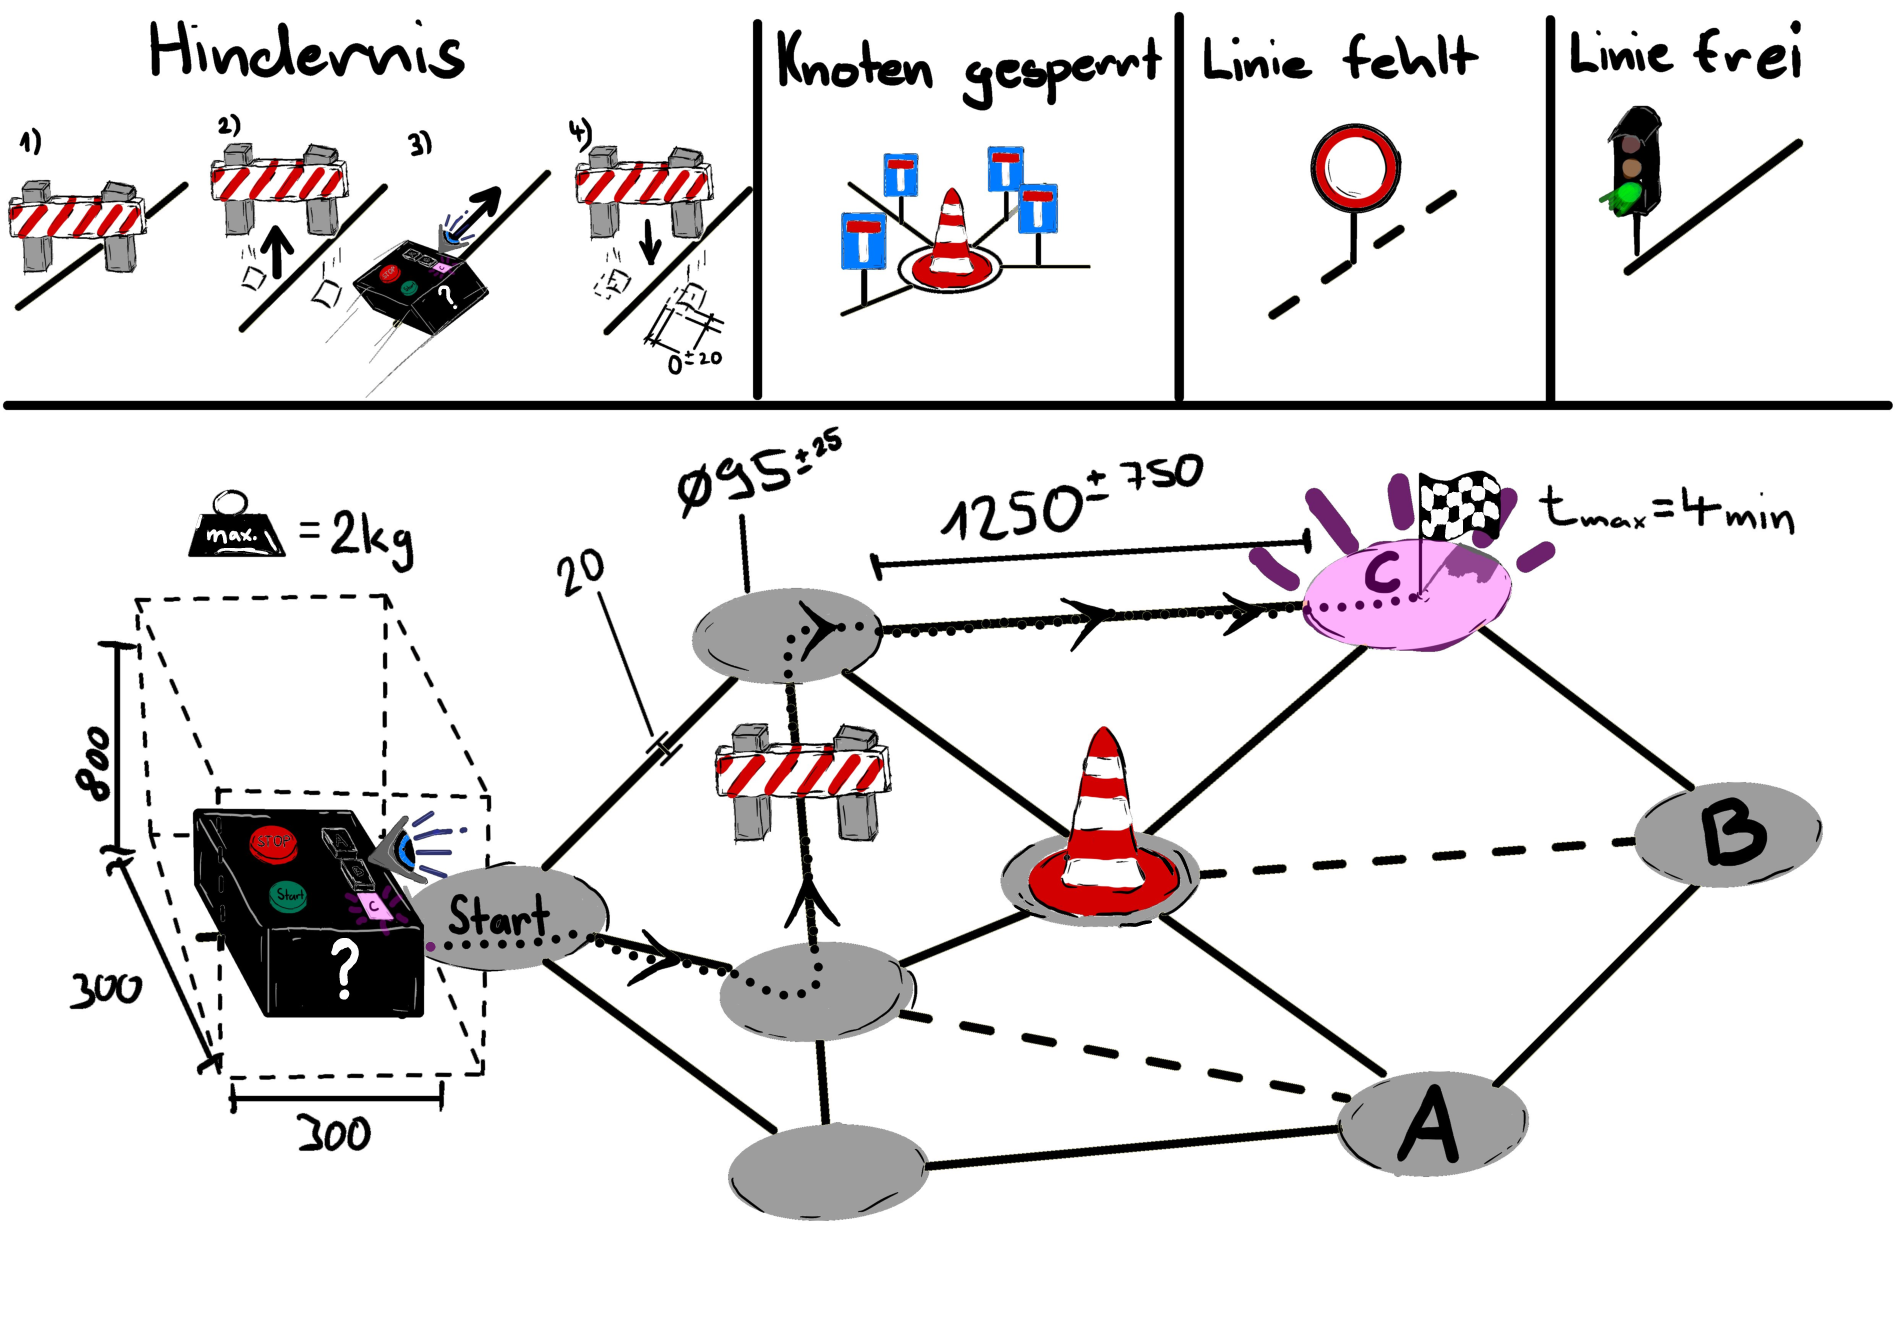
\includegraphics[width=\textwidth]{img/Skizze_Aufgabenstellung_v4.2.png}
\caption{Aufgabenstellung}
\label{fig:aufgebanstellung}
\end{figure}

\subsection{Anforderungsliste}

Die Anforderungsliste wurde basierend auf der Aufgabenstellung erstellt und anschliessend von dem betreuenden Dozenten freigegeben. Zur Strukturierung wurden die Anforderungen in sieben Gruppen gegliedert: Gerät, Sicherheit, Software, Nachhaltigkeit, Demonstration, Wegenetz und Budget. Die einzelnen Anforderungen wurden in die Kategorien Fest-, Mindest-- und Wunschanforderungen unterteilt. Zu jeder Anforderung wurde mindestens eine Fachrichtung definiert, welche für die Einhaltung der
Anforderung verantwortlich ist.

Die vollständige Anforderungsliste befindet sich im Anhang im Kapitel \nameref{anforderungliste}.